\documentclass{beamer}

\usepackage[utf8]{inputenc}

\usetheme[navigation]{UMONS}

\title{ma partie}
\author{Antoine}
\date{}

\institute[]{%
  Faculté des Sciences\\
  Université de Mons
  \\[1cm]
  \includegraphics[height=5ex]{UMONS}\hspace{2em}%
  \raisebox{-1ex}{\includegraphics[height=10ex]{UMONS_FS}}
  \\
  \vspace{2ex}
}




\begin{document}

\begin{frame}[plain]
    \titlepage
\end{frame}

\begin{frame}[plain]
    \frametitle{Un petit peu de magie\dots~pas trop}

   Qu'est-ce que l'exemple du tour de magie nous apprend ? 

   Au départ, on a plein d'hypotèses sur l'explication :

   \begin{itemize}
       \item il se passe vraiment un truc magique, ou alors
       \item il y a une manipulation ultra complexe des cartes, ou alors
       \item il a lu dans l'esprit des participants pour voir comment ils allaient placer leurs cartes
       \item \dots
   \end{itemize}

   \pause

   Après on refait le tour et nos hypothèses changent

   \begin{itemize}
       \item Il y a de très très très grosses chances que ça donne toujours le même résultat
       \item mais peut-être que c'est le hasard et qu'il manipule bien les cartes
       \item ou alors il lit dans nos esprits mais j'en doute
       \item \dots
   \end{itemize}

   

\end{frame}

\begin{frame}[plain]
    \frametitle{La reproductibilité}

\onslide<1-3>{De toute évidence, c'est difficile d'expérimenter si une évènement ne se produit qu'une fois} 

\vspace{1cm}

\onslide<2-3>{\alert{$\rightarrow$} la science s'intéresse aux phénomènes reproductibles}

\vspace{1cm}

\onslide<3>{Comment on pourrait appeler un évènement qui ne se produirait qu'une fois ?}

\end{frame}

\begin{frame}[plain]

\onslide<1>{\centering
\includegraphics[scale=.9]{images/miracle.jpg}}

\end{frame}


\begin{frame}[plain]
    \frametitle{La reproductibilité}

\onslide<1->{Si un miracle se reproduit, ça n'est plus un miracle.}

\vspace{1cm}

\onslide<2->{Imaginez qu'un gars ressuscite des gens. Au début ça étonnera, mais si il le fait tous les trois jours, on commencera à essayer de savoir comment il fait \alert{$\rightarrow$} C'est là que la science commence.}

\vspace{1cm}

\onslide<3->{En fait, un miracle, c'est ce qui va à l'encontre des \alert{lois naturelles}.}

\end{frame}

\begin{frame}[plain]
    \frametitle{Niveaux de preuve : pourquoi l'extraordinaire est plus difficile à croire (et pourquoi c'est plutôt bien comme ça) ?}

    Dans le cas du tour de magie, le fait qu'on s'habitue au résultat nous a fait revoir notre évaluation de la situation. \pause

    \vspace{1cm}

    \textit{Une affirmation extraordinaire requiert des preuves extraordinaires} \pause \alert{$\rightarrow$} On évalue la valeur d'une preuve en comparaison avec les éléments qui vont dans l'autre sens. \pause

    \vspace{1cm}

    Pour croire à un miracle, il faudrait que l'impossibilité du miracle soit plus miraculeuse que son déroulement.


\end{frame}

\begin{frame}[plain]
    \frametitle{Rasoir d'Ockham}

    Toutes choses étant égales par ailleurs, il est rationnel de privilégier l'explication la plus simple.\pause

    \vspace{1cm}

    Face à un fait nouveau, l'explication ne doit pas soulever plus d'inconnues que le fait de départ.\pause

    \vspace{1cm}

    C'est exactement ce qu'on avait tendance à faire dans le cas du tour de magie.



\end{frame}

\begin{frame}[plain]
    \frametitle{Des dragons et des chats}

    \onslide<1-3>{Mon voisin me dit : \textit{Il y a un dragon dans mon garage}.}

    \onslide<2-3>{\vspace{1cm}

    C'est plutôt extraordinaire, donc ça demande une preuve plus grande que son simple témoignage}

    \onslide<3>{\vspace{1cm}

    Et ses explications doivent être plus parcimonieuses que le fait qu'il propose}

\end{frame}

\begin{frame}[plain]

    \vspace{-1cm}\centering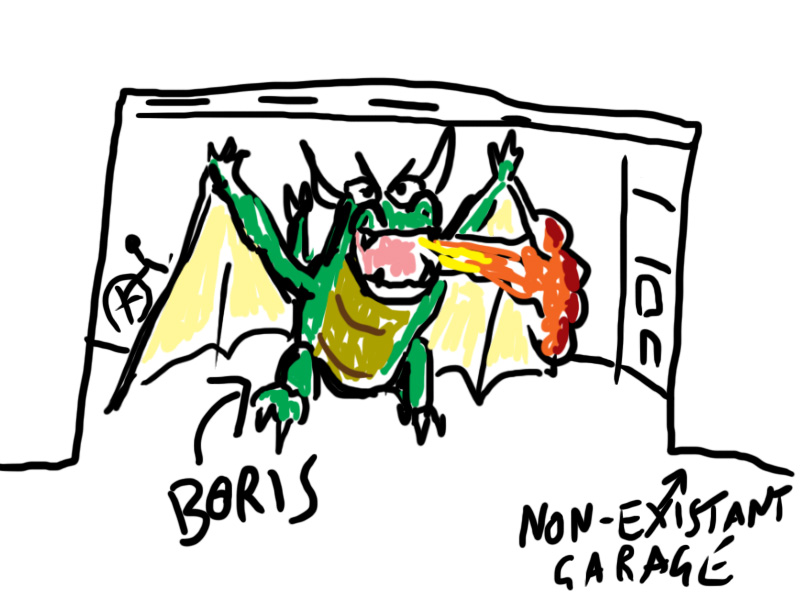
\includegraphics[scale=.4]{images/dragon.jpg}

\end{frame}

\begin{frame}[plain]
    \frametitle{Le chat dans la boîte}

    \only<1->{Expérience de haut-vol : vous mettez un chat et une souris dans une boîte opaque. Dix minutes plus tard vous revenez : il n'y a plus que le chat.}

    \begin{itemize}
            \item<2-> la souris s'est transformée en gaz et s'est évaporée à travers la boîte
            \item<3-> la souris est passée à travers la paroi par effet tunnel quantique
            \item<4-> le chat a mangé la souris
            \item<5-> la souris a mangé le chat, puis s'est transformée en chat
    \end{itemize}

    \vspace{.5cm} 
    
    \only<1->{\centering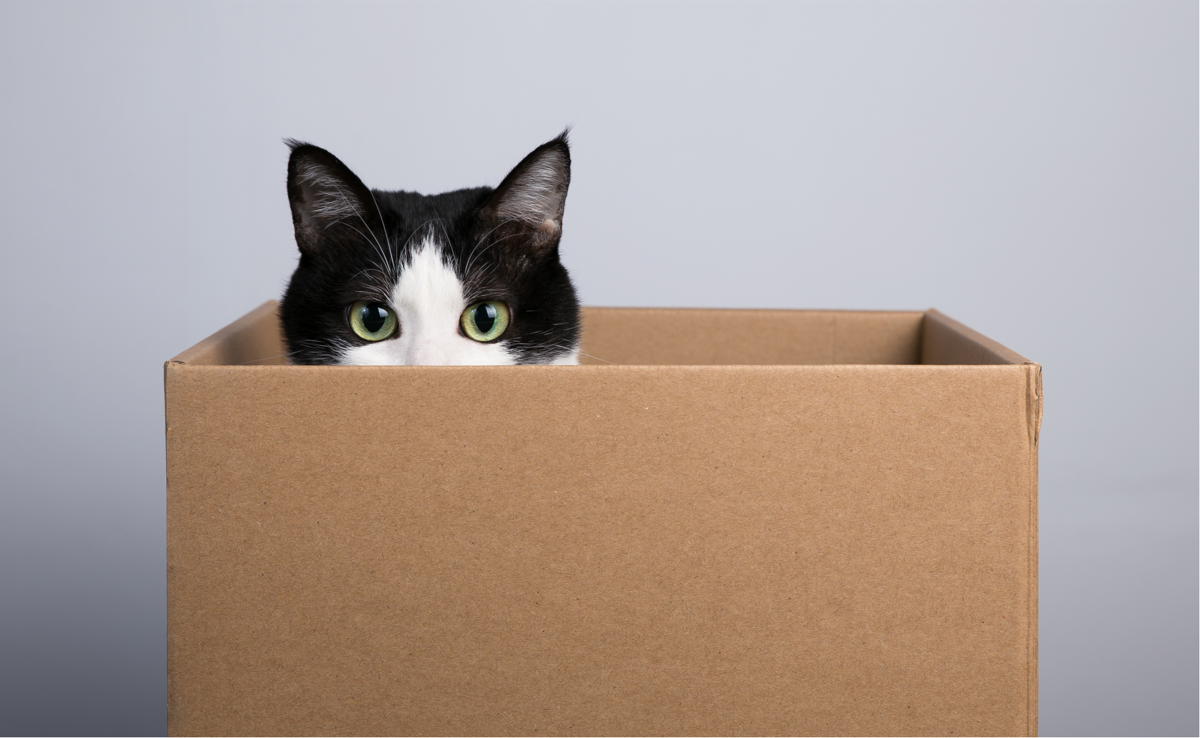
\includegraphics[scale=.6]{images/chat.png}}

\end{frame}

\end{document}
